\chapter{The Proposed Approach}\label{sec:approach}

\begin{figure*}[ht!]
\centering
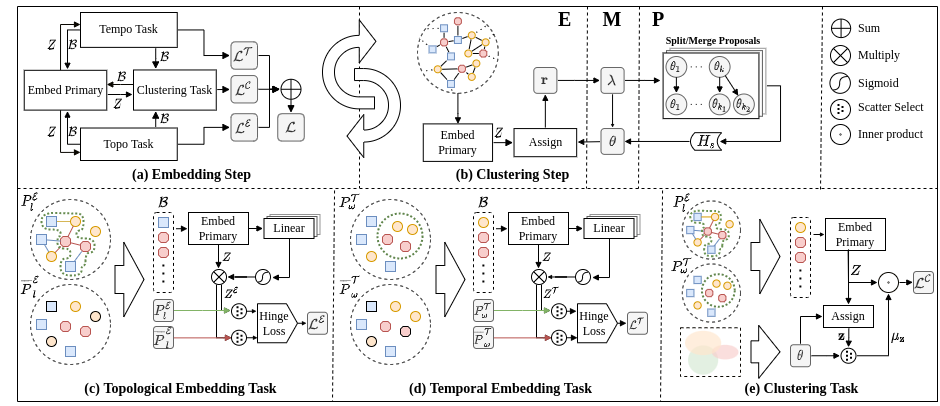
\includegraphics[width=\textwidth]{resources/framework.png}
\caption{Overview of the MGTCOM framework.
(a) In the embedding step primary embeddings are used in auxiliary tasks to construct the multi-objective loss. 
(b) Clustering step updates clustering by alternating between Expectation (\textbf{E}), Maximization (\textbf{M}), and Proposal (\textbf{P}) steps.
(c) In the topological (topo) embedding task, random walk sampling and feature-wise attention minimize inter-node proximity.
(d) In the temporal (tempo) embedding task, ballroom walk sampling and feature-wise attention minimize proximity between temporally related nodes.
(e) Clustering task adds community awareness to the embeddings by minimizing proximity between nodes within the same cluster.
}
\label{fig:framework}
\end{figure*}

We present our framework for Community Detection in Temporal Multimodal Graphs (MGTCOM) that learns multimodal representation vectors for graph nodes and detects communities in tandem.
We achieve this by leveraging heterogeneous graph transformers \cite{huHeterogeneousGraphTransformer2020} to learn a primary node embedding function $\zeta$. In order to handle the incompleteness constraints, we introduce an auxiliary embedding vector $E$ for known (or seen) nodes with missing features.
Next, we learn task-specific node representation for topological and temporal information by combining primary embeddings with task-specific transformation/attention and context sampling. 
As we utilize random walks for topological context sampling, we introduce its analogue as an unbiased temporal window sampling algorithm for temporal context collection.
Finally, we adopt DPMM for community detection and close the loop by introducing cluster-based loss to ensure the graph embeddings are \textit{community-aware}.
%
MGTCOM consists of three major components (as can be seen in \cref{fig:framework}): primary embedding module, (a) task-specific learning, and (b) community detection/clustering module. MGTCOM also has a graph sampling component.  In the following, we describe the components in detail. 

\section{Primary embedding module}
The central component of our framework is responsible for inferring the primary representation vector $Z_v$ given a node $v \in \mathcal{V}$ in a graph $G$. 
%
Motivated by the success of inductive GCN-based methods \cite{hamiltonInductiveRepresentationLearning2017, yingGraphConvolutionalNeural2018, huHeterogeneousGraphTransformer2020}, we build our architecture by combining $L$ graph convolution layers ($\mathit{HeteroConv}$ or HGCN) and a graph subsampler ($\mathit{HeteroSample}$). 

Specifically, we use the budget-based subgraph sampling algorithm and the heterogeneous graph transformer (HGT) proposed by Hu et al. \cite{huangInformationFusionOriented2022}.
HGT captures topological, meta-topological, and content-based aspects by combining off-the-shelf graph convolution with node type-specific projection and edge type-based attention.

\cref{alg:prim_feat} provides a full overview of the primary embedding algorithm. 
The basic idea is to infer node representation from its k-hop heterogeneous neighborhood subgraph $G_v$ while handling edge cases introduced by the incompleteness constraints (\cref{def:incompleteness_constraints}) in order to handle web-scale multimodal graphs.
The inference starts by sampling a subgraph $G_{\mathcal{B}}$ given a batch of central nodes using the \textit{budget sampling} algorithm on \cref{alg:pe:sampling}.
The \textit{budget sampling} algorithm works by restricting sampled subgraph at each layer given a per node type limit.
For our use case, we define this limit as multiple $|\mathcal{B}|$ to avoid re-tuning its value for each dataset. 
% We use node type bound budget required by \textit{budget sampling} algorithm as a multiple of $|\mathcal{B}|$ for each of the layers to hyperparameter retuning for different datasets.

Once the graph is sampled we split the task of initial feature inference into three cases to handle the incompleteness constraints.
(i) If a feature vector is present, then it is simply projected into the representation space.
(ii) If the node is in the training set while no feature vector is present, then its representation is drawn from the \textit{auxiliary embedding} matrix $\mathbf{E}$. To avoid overreliance on the embeddings in preference for feature vectors we apply dropout on the resulting representation.
(iii) Finally, if an unseen node without a feature vector is encountered, the zero vector (denoted as $0_d$) is used, indicating that its feature vector has zero weight during the aggregation step of the graph convolution.
Note that for large datasets, it may not be feasible to keep a full auxiliary embedding matrix in memory. 
In \cref{sec:abl:aux_emb} we explore a setting where auxiliary embeddings are limited to a subset of important nodes.

\begin{algorithm}[!t]
    \small
    \caption{Batchwise primary node embedding}\label{alg:prim_feat}
    \SetKwFunction{procPrimary}{EmbedPrimary}

    \SetKwProg{myproc}{Procedure}{}{}
    \myproc{\procPrimary{}}{
        \KwIn {
            multimodal graph $G = (\mathcal{V}, \mathcal{E}, \mathcal{A}, \mathcal{R}, \mathcal{X})$,
            mini-batch $\mathcal{B} \subseteq \mathcal{V}$,
            auxiliary node embedding $\mathbf{E} \in \mathbb{R}^{N_{\bar{\mathcal{X}}} \times d }$
            where $N_{\bar{\mathcal{X}}} = |\{v|v \in \mathcal{V}, \mathbf{1}_{\mathcal{X}}(v) = 0\}|$,
            number of convolutional layers $L$
        }
        \KwOut {
            The primary embedding $Z_{\mathcal{B}}$ for nodes in batch $\mathcal{B}$
        }
            $G_{\mathcal{B}}(\mathcal{V}_{\mathcal{B}}, \mathcal{E}_{\mathcal{B}}, \mathcal{A}_{\mathcal{B}}, \mathcal{R}_{\mathcal{B}}, \mathcal{X}_{\mathcal{B}}) \leftarrow \operatorname{HeteroSample}(G, \mathcal{B}, L)$\; \label{alg:pe:sampling}
            \For {$s \in \mathcal{V}_{\mathcal{B}}$} {
                $H_s^{(0)} = \begin{cases}
                    \operatorname{Linear}(\mathbf{x_s}) & \mathbf{1}_{\mathcal{X}}(s) = 1 \\
                    \operatorname{Dropout}(\mathbf{E}_s)& \mathbf{1}_{\mathcal{V}}(s) = 1 \\
                    0_d                                 & \text{otherwise}
                \end{cases}$\; \label{alg:pe:feature_inf}
            }
            \For {$l = 1$ \KwTo $L$} {
                $H^{(l)} = \operatorname{GeLU}(\operatorname{HeteroConv}(G_{\mathcal{B}}, H^{(l-1)}))$\; \label{alg:pe:conv}
            }
            $Z_{\mathcal{B}} = \{H^{(L)}_t | t \in \mathcal{B} \}$\; \label{alg:pe:batch}
        \Return {$Z_{\mathcal{B}}$}
    }
\end{algorithm}


On \cref{alg:pe:conv}, given the subgraph $G_\mathcal{B}$ and the initial representation vector $H^{(0)}$,  $L$ layers of HGT graph convolutions are applied.
Each layer uses the representation vector of the previous layer and feeds its output through a $\operatorname{GeLU}$ \cite{hendrycksGaussianErrorLinear2020} activation function (See \cref{sec:abl:hyperparam} for performance comparison).
Finally, the output vectors at the $L^\mathit{th}$ layer are used as primary representation vectors and output for each query node in the batch on \cref{alg:pe:batch}. 

\section{Multi-task representation learning}
During task-specific learning we focus on two main tasks capturing the intricacies of multimodal networks.
The topological task identified by $\mathcal{E}$ focuses on minimizing the representation distance between nodes that are proximate within the network.
Analogously, the temporal task $\mathcal{T}$ focuses on minimizing the distance between nodes that co-occur at the same timeframes.
While fundamentally different since the tasks are trained in parallel, they benefit from weight sharing and from node sharing during primary embedding as the subgraph batches are centered around the same nodes.

\subsection{Task-based attention}
An important observation is that while temporal and topological communities are both important during analysis, they are not always correlated.
In fact, in most of the benchmarking datasets such as Cora and DBLP temporal features and graph structure show low correlation.
While it is very rare that contentual features are completely independent of topology and temporality, we describe a general implementation that can be applied to such a case. 

Given the above observation, we admit that it may not be possible to train a model that excels at both tasks.
To work around this issue while still capturing both tasks in a single embedding vector we introduce \textit{task-based attention}.
The basic idea is that while primary embedding extracts suitable features from the multimodal network, task-specific attention selects the most relevant of these features for the task at hand.
%
Inspired by transformers \cite{vaswaniAttentionAllYou2017} we define multi-head attention to capture various feature patterns \cref{eq:task_attention}.
The task-based transformation function is defined as \cref{eq:task_transform} where the primary representation vector is attended to using a simple matrix multiplication operation.
We specialize this function for topological task as $f^{\mathcal{E}}(\mathbf{Z})$ producing $\mathbf{Z}^{\mathcal{E}}$ and temporal task $f^{\mathcal{T}}(\mathbf{Z})$ producing $\mathbf{Z}^{\mathcal{T}}$.

\begin{align}
    f^{task}(\mathbf{Z}) &= \mathbf{Z} \cdot \operatorname{\textit{ATT}}^{task}(\mathbf{Z}) \label{eq:task_transform}  \\
    \operatorname{\textit{ATT}}^{task}(\mathbf{Z}) &= \underset{i \in [1..h]}{\|} \sigma \left[ \operatorname{Linear}^i_{task}(\mathbf{Z}) \right] \label{eq:task_attention}
\end{align}

\subsection{Objective function} \label{sec:obj_fn}
In order to learn model parameters in an unsupervised way, we define contrastive loss.
Task-specific positive context sample $P$ and a negative context sample $\bar{P}$, both sharing a central query node $q$ are used to construct positive $(q, p)$ and negative $(q, n)$ node pairs respectively.
We define a max-margin-based loss function (\cref{eq:max_margin}) which aims to maximize the inner product similarity between the query and positive examples.
On the other hand, the inner product of query and negative samples is minimized to be smaller than that of the positive samples by some predefined value of $\Delta$ (see \cref{sec:abl:hyperparam} hyperparameter experiments).
In our tests, we found that averaging similarity over positive samples within the max loop helps to smoothen out the noise caused by context sampling \cref{eq:mm_mean_aff}.

\begin{align}
    \operatorname{MM-Loss}(\mathbf{Z}, P, \bar{P}, q) &= \max_{n \in \bar{P}} \left\{0, \mathbf{Z}_q \mathbf{Z}_n - \widetilde{\mathbf{Z}_q \mathbf{Z}_p} + \Delta \right\} \label{eq:max_margin} \\
    \widetilde{\mathbf{Z}_q \mathbf{Z}_p} &= \frac{1}{|P|} \sum_{p \in P } \left(\mathbf{Z}_q \mathbf{Z}_p \right) \label{eq:mm_mean_aff}
\end{align}

% ====================================
\subsection{Temporal context sampling}\label{sec:tempo_sampling}
\begin{figure*}[htbp]
\centering
\subfigure[]{
% 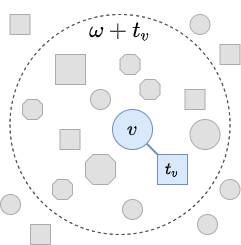
\includegraphics[width=0.42\columnwidth]{resources/ballroom/br2.png}
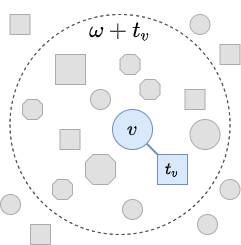
\includegraphics[width=0.21\columnwidth]{resources/ballroom/br2.png}
}\quad
\subfigure[]{
% 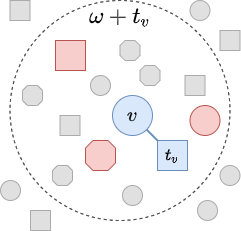
\includegraphics[width=0.42\columnwidth]{resources/ballroom/br3.png}
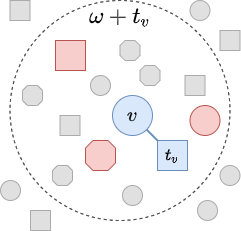
\includegraphics[width=0.21\columnwidth]{resources/ballroom/br3.png}
}\quad
\subfigure[]{
% 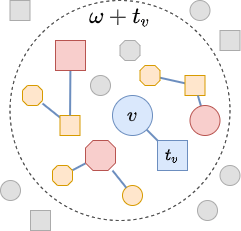
\includegraphics[width=0.42\columnwidth]{resources/ballroom/br4.png}
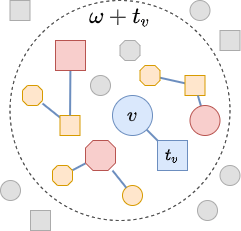
\includegraphics[width=0.21\columnwidth]{resources/ballroom/br4.png}
}\quad
\subfigure[]{
% 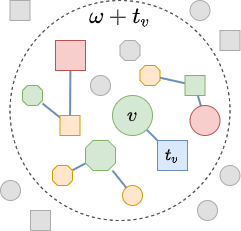
\includegraphics[width=0.42\columnwidth]{resources/ballroom/br5.png}
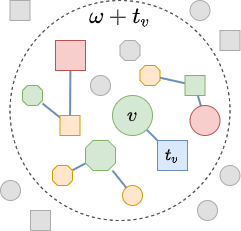
\includegraphics[width=0.21\columnwidth]{resources/ballroom/br5.png}
}\quad

\caption{
    Visual overview of Ballroom Walk temporal sampling algorithm.
    (a) The sampling timestamp $t_v$ for query node $v$ is inferred given the nearest neighbor if the node is static (blue). The relative time window is determined as $\omega + t_v$.
    (b) The root context nodes are sampled from the relative time window (red).
    (c) Context is extended with temporal random walks from the root nodes (yellow).
    (d) The context path is sampled from the collected context (green).
}
\label{fig:br}
\end{figure*}

Temporal features are often not correlated with network topology.
We propose a separate context sampling function that, given a query node and an interval window $\omega$, returns other nodes occurring within the same time window. 
The interval window $\omega$ is determined by using the dataset statistics as a fraction of the complete time range $\mathcal{T}$.
By picking a small enough interval window, a fine-grained continuous-time representation vector can be learned.
This is because additional granularity is achieved by centering the sample around the query node.
% as during sampling it is shifted to be centered around the query node.

Edge cases arising from the incompleteness constraints need to be handled where the nodes are missing timestamps $\mathbf{1}_{\mathcal{T}} = 1$.
While the usual semantic approach is to consider these nodes omnipresent (static), the naive window sampling methods quickly get congested with static to static context pairs.
Our aim is to alleviate this issue using biased sampling in favor of non-static pairs.

We start by introducing the temporal random walk procedure shown in \cref{alg:tempo_rw} which enforces standard random walks over the network to stay within a predetermined temporal window $\omega^*$.
Here random walk of size $l$ is constructed by picking a randomly connected node to the current head node (\cref{alg:trw:neighbors}) within a time window.
If no such node is present, then the random walk is restarted from any already picked node \cref{alg:trw:restart}.
The walk is extended with a new head node until it reaches the desired length.

\begin{algorithm}[!t]
    \small
    \caption{Temporal Random Walk}\label{alg:tempo_rw}
    \SetKwFunction{algo}{BallroomWalk}
    \SetKwFunction{proc}{TemporalRW}
    \SetKw{KwGoTo}{go to}
    
    \setcounter{AlgoLine}{0}
    \SetKwProg{myproc}{Procedure}{}{}
    \myproc{\proc{}}{
    \KwIn {
        center node $v$,
        temporal window $\omega^*$
    }
    \KwOut {
        Temporal random walk $P_l$
    }
        Initialize $P_l$ = $[]$\; 
        $(u, t_u) = (v, \varnothing)$\;
        \For {$i = 1$ \KwTo $l$} {
            $N(u) = \{w| 
                w \in \mathcal{V}, 
                (u, w) \in \mathcal{E},
                \tau(w) \cap \omega^* \neq \emptyset
            \}$\;\label{alg:trw:neighbors}
        
            \If (\tcc*[h]{Restart on dead end}){$N(u) = \emptyset$}{
                $(u, t_u) = (v, t_v)$\; \label{alg:trw:restart}
                \KwGoTo \ref{alg:trw:neighbors}\;
            }

            $w \sim N(u)$\; \label{alg:trw:sample}
            $t_u = \max \left\{ t_u, \min{ \tau(w)} \right\}$\;
            $u = w$\;

            $P_{l}.append((u, u_t))$\;
        }

        \KwRet $P_l$
    }
\end{algorithm}

Utilizing the idea of temporal random walks we propose our own sampling method "Ballroom Walk" whose outline is shown in \cref{alg:ballroom_walk}.
% An outline of our proposed sampling method "Ballroom Walk" is shown in \cref{alg:ballroom_walk}.
It starts by inferring the sampling timestamp $t_v$ by picking a random timestamp the query node $v$ occurs in.
If the node is static, the timestamp of its nearest neighbor reachable through temporal random walk is selected (\cref{alg:brw:infer_t}).
To reliably sample the temporal neighborhood, $n$ root nodes ($w$) are picked occurring in the time-window relative to the sampling timestamp on \cref{alg:brw:neighborhood}.
Temporal context $C$ is constructed by collecting temporal random walks starting from root nodes $w$ given a relative time window $\omega + t_v$ on \cref{alg:brw:context}.
Finally, $l$ long context paths are created as random subsets of $C$.
Note that because a sampled context is valid for all member nodes, random walk-like throughput optimization can be used by setting a larger window length than context size~\cite{perozziDeepWalkOnlineLearning2014}.

\begin{algorithm}[!t]
    \small
    \caption{Ballroom walk sampling}\label{alg:ballroom_walk}
    \SetKwFunction{algo}{BallroomWalk}
    \SetKwFunction{proc}{TemporalRW}
    \SetKw{KwGoTo}{go to}
    
    \SetKwProg{myalg}{Algorithm}{}{}
    \myalg{\algo{}}{
    \KwIn {
        %temporal graph $G = (\mathcal{V}, \mathcal{E}, \mathcal{T})$,
        multimodal graph $G = (\mathcal{V}, \mathcal{E}, \mathcal{A}, \mathcal{R}, \mathcal{X})$,
        relative temporal window $\omega$,
        walks per node $n$,
        walk length $l$,
        center node $v$, 
    }
    \KwOut {
        Temporal $n$ random walks $P_l$
    }
        Initialize $C$\;
        $t_v = \begin{cases}
            t_v \sim \tau(v)                                            & \mathbf{1}_{\mathcal{T}}(v) = 1 \\
            % [(\_, t_v), ...] \leftarrow \proc{$v$, $(-\infty, \infty)$}     & \text{otherwise}
            \proc{$v$, $(-\infty, \infty)$}.first()     & \text{otherwise}
        \end{cases}$\; \label{alg:brw:infer_t}
        $N(v) = \{w|
            w \in \mathcal{V}, 
            \tau(w) \cap \omega + t_v \neq \emptyset
        \}$\; \label{alg:brw:neighborhood}
        \For {$i = 1$ \KwTo $n$}{
            $w \sim \mathcal{N}$\;
            $C = C \cup \proc{$w$, $\omega + v_t$}$\; \label{alg:brw:context}
        }
        \texttt{RandomPermute}($C$)\;

        \For {$i = 1$ \KwTo $n$}{
            $P_l = \{C_j | i \cdot l \leq j < i \cdot l+l\}$\; \label{alg:brw:walks}
            \KwRet $P_l$\;
        }
    }{}
    
    % \setcounter{AlgoLine}{0}
    % \SetKwProg{myproc}{Procedure}{}{}
    % \myproc{\proc{}}{
    % \KwIn {
    %     center node $v$,
    %     temporal window $\omega$
    % }
    % \KwOut {
    %     Temporal random walk $P_l$
    % }
    %     Initialize $P_l$\; 
    %     $(u, t_u) = (v, \varnothing)$\;
    %     \For {$i = 1$ \KwTo $l$} {
    %         $\mathcal{N} = \{w| 
    %             w \in \mathcal{V}, 
    %             (u, w) \in \mathcal{E},
    %             (\tau(u) \cap \tau(w) \cap \omega ) \neq \emptyset
    %         \}$\;\label{all:tempo_neighbors}
        
    %         \If (\tcc*[h]{Restart on dead end}){$\mathcal{N} = \emptyset$}{
    %             $(u, t_u) = (v, t_v)$\;
    %             \KwGoTo \ref{all:tempo_neighbors}\;
    %         }

    %         $w \sim \mathcal{N}$\;
    %         $t_u = \max \left\{ t_u, \min \tau(w), \tau((u, w)) \right\}$\;
    %         $u = w$\;

    %         $P_{l}.push((u, u_t))$\;
    %     }

    %     \KwRet $P_l$
    % }
\end{algorithm}

Due to timestamp inference, the first- and second-order proximity static to static pairs are ignored.
By only passively sampling omnipresent nodes we mitigate the over-saturation issue while still being fair.
Most importantly the neighborhood of central nodes is being sampled independently of their topology.
By sampling within a temporal window, we avoid not relying on the correlation of temporality with topology.

% ====================================
\subsection{Graph sampling}
The objective of task-specific learning is mainly defined by the context sampling method.
As our method allows for inference of primary and task-specific representations for unseen nodes, we assume that topological, meta-topological and contentual features contain enough information / are correlated with the objective of the tasks.
%
% Topo sampling
To gather the topological context $P^{\mathcal{E}}$, Node2Vec biased random-walk algorithm is utilized \cite{groverNode2vecScalableFeature2016}.
By choosing a low value for its control parameter $q$ we discourage structural/topological equivalence representation in favor of larger neighborhood exploration (depth-first strategy) which is useful for community representation.
% Tempo sampling
Similarly, we use ballroom sampling to collect temporal context $P^{\mathcal{T}}$ of size $l$ as introduced in the previous section.
The negative nodes are collected by sampling random nodes from the graph.
% Sharing
In our framework, the query nodes and negative contexts are shared across both tasks. 
% Similarly, as the tasks are trained in parallel, their loss is combined to facilitate multi-objective optimization (See \cref{alg:pipeline}).

\section{Community detection}
For community detection, we adopt the DPMM split/merge algorithm proposed by Chang and Fisher III \cite{changParallelSamplingDP2013a} as discussed in \cref{sec:dpmm}.
In our implementation, we use Normal Wishart (NW) as a conjugate prior and use variational lower bound in our convergence criteria.
%
Specifically, we monitor the log sum of the variational lower bound \cref{eq:var_lb} for the supercluster and subcluster models. 
The variational lower bound is computed as the product of variational distribution $q(\mathbf{z})$, the normalizing constant of the Dirichlet distribution $B(\alpha_0)$, and the normalizing constant of the Normal Wishart distribution $C(W, \nu)$.
Once its monitored value starts oscillating, then the model has converged and is moved into the proposal state.
If the model parameters remain unchanged during the proposal stage (no split or merge is accepted), then the clustering is complete.

\begin{align}
    \operatorname{Lower-Bound}(r) = 
    \underbrace{\left[ \prod_{n=1}^{N} \prod_{k=1}^K r_{nk} e^{r_{nk}} \right]}_{q(\mathbf{z})}
    \underbrace{\frac{\prod_{i=1}^K \Gamma(\alpha_0)}{\Gamma \left( \sum_{k=1}^K \alpha_0 \right)}}_{B(\alpha_0)}
    \underbrace{2^{\frac{\nu d}{2}} |W|^{\frac{\nu}{2}} \Gamma_d \left(\frac{\nu}{2} \right)}_{C(W, \nu)} \label{eq:var_lb}
\end{align}

The only parameters relevant for our clustering method are the prior hyperparameters (See \cref{sec:dpmm}).
Most of the parameters (i.e. $\alpha$, $\kappa$, and $\nu$) are not very relevant if they are much smaller than the sample count.
We use the $\Sigma_{scale}$ parameter to scale the dataset covariance for more effective control over the strength of the data-bound prior parameters $\mu_0, \Sigma_0$.
In \cref{sec:abl:hyperparam} we provide a more detailed analysis of result sensitivity to prior parameters.

To fit the clustering model we use primary embedding to calculate assignment and posterior parameters as it contains features relevant for both temporal and topological tasks.
While not explored in this thesis, it is worth noting that it is not necessary to have all the embeddings in memory as exact posterior parameters depend on data $\mu$ and $\Sigma$ which can be calculated over multiple batches.

\section{End-to-end approach}
Given a graph embedding, it is straightforward to find communities by performing the embedding and clustering tasks sequentially. 
This approach lacks a unified objective, thus, the node embeddings may not be optimized for community detection.
We extend the objective with cluster-based loss calculated as the distance between node embedding and its assigned cluster $z_v$ \cref{eq:loss_clus}.
This introduces a feedback loop that encourages the model to reinforce community structures while optimizing the topological and temporal objectives \cref{eq:combined_loss}.
%
The influence of three objectives can be controlled using hyperparameters $\beta^{\mathcal{E}}$, $\beta^{\mathcal{T}}$, and $\beta^{\mathcal{C}}$.

\begin{align}
    \mathcal{L}^{C} &= \left\|Z_v - \mu_{z_v} \right\|^2_{\ell 2} \label{eq:loss_clus} \\
    \mathcal{L}^{\mathcal{E}} &= \operatorname{MM-Loss}(\mathbf{Z}, P^{\mathcal{E}}, \bar{P}, v) \label{eq:loss_topo} \\
    \mathcal{L}^{\mathcal{T}} &= \operatorname{MM-Loss}(\mathbf{Z}, P^{\mathcal{T}}, \bar{P}, v) \label{eq:loss_tempo}\\
    \mathcal{L} &= \beta^{\mathcal{E}} \mathcal{L}^{\mathcal{E}} + \beta^{\mathcal{T}} \mathcal{L}^{\mathcal{T}} + \beta^{\mathcal{C}} \mathcal{L}^{\mathcal{C}} \label{eq:combined_loss}
\end{align}


With this closed feedback loop, the training procedure consists of two alternating stages (See \cref{fig:framework} and \cref{alg:pipeline}).
The \textit{embedding optimization} stage (\cref{alg:pipeline:feat_optimization}), is responsible for optimizing the graph embedding function parameters while keeping cluster parameters $\theta$ fixed.
Once the graph embeddings are updated we run $I_c$ clustering/EM steps to optimize cluster parameters $\theta$ while keeping node representations fixed \cref{alg:pipeline:cluster_optimization}. Note that the \textit{representation optimization} stage is run until convergence as part of pretraining beforehand to ensure the clusters are initialized properly.

\begin{algorithm}[t!]
    \small
    \caption{MGTCOM learning pipeline}\label{alg:pipeline}
    \For {$subiter = 1$ \KwTo $I$}{
        \For {$v \in \mathcal{V}$}{ \label{alg:pipeline:feat_optimization}
            \tcc{Gather context samples}
            $P^{\mathcal{E}} = \texttt{Node2VecRandomWalk}(G, l, v)$\;
            $P^{\mathcal{T}} = \texttt{BallroomWalk}(G, \omega, l, v)$\; %\algo{$G$, $\omega$, $l$, $v$}$\;
            % $\bar{P}_l = \{w \sim \mathcal{V}| \text{for} i \in [1..l] \}$ \tcc{Negative sampling}
            $\overline{P} \stackrel l\sim \mathcal{V}$ Negative sampling\;
            $\mathcal{B} = P_l^{\mathcal{E}} \cup P_l^{\mathcal{T}} \cup \bar{P}_l$\;
            $\mathbf{Z} = \procPrimary{$G$, $\mathcal{B}$}$\;
            Compute task embeddings $Z^{\mathcal{E}}$, $Z^{\mathcal{T}}$ using \cref{eq:task_transform}\;
            Compute loss $\mathcal{L}^{\mathcal{E}}$, $\mathcal{L}^{\mathcal{T}}$, $\mathcal{L}^{\mathcal{C}}$, $\mathcal{L}$ using \cref{eq:loss_clus,eq:loss_topo,eq:loss_tempo,eq:combined_loss} given respective context $P^{\mathcal{E}}$, $P^{\mathcal{T}}$\;
        }
        \For {$iter = 1$ \KwTo $I_c$}{ \label{alg:pipeline:cluster_optimization}
            \If {$i = 1$}{
                Initialize $\theta$ using K-means
            }
            Update $\theta$ using EM given $Z$
        }
    }
  % \Return {$\theta$}
\end{algorithm}
